\documentclass[a4paper,11pt,openright,openbib]{article}
\usepackage[portuges]{babel}
\usepackage[T1]{fontenc}
\usepackage{ae}
\usepackage[utf8]{inputenc}
\usepackage[pdftex]{graphicx}
\usepackage{url}
\usepackage{listings}
\usepackage{verbatim}
\usepackage{enumerate}
\usepackage{epstopdf}
\usepackage[a4paper, pdftex, bookmarks, colorlinks, linkcolor=black, urlcolor=blue]{hyperref} 
\usepackage[a4paper,left=2.5cm,right=2.5cm,top=3.5cm,bottom=3.5cm]{geometry}
\usepackage{colortbl}
\usepackage[margin=10pt,font=small,labelfont=bf]{caption}
\usepackage{mdwlist}


\setlength{\parindent}{0cm}
\setlength{\parskip}{2pt}




\title{
	\large{
\includegraphics[width=0.3\textwidth]{../../report-template/UM.jpg}} \\
	\large{Universidade do Minho}  \\
	\large{Mestrado em Engenharia Informática}  \\
	\large{Engenharia de Linguagens}  \\
	\large{Projecto Integrado - Grupo 1}  \\	
	\large{\textbf{2ª Avaliação Intermédia}} \\
	\large{Ano Letivo de 2012/2013} \\
	\date{\today}
}

\author{	
	\begin{tabular}[t]{c c}      
        pg22820 - \textbf{António Silva} \\        
	pg22781 - \textbf{Rui Brito} \\   				
	\\ 
	\end{tabular}
}

\begin{document}

\maketitle


\pagestyle{headings}
\pagenumbering{arabic}
\newpage
\tableofcontents
\newpage

\section{Introdução}
O projecto consiste no desenvolvimento de um sistema de informação que permita gerir os dados curriculares de um docente universitário.\\
Essa informação a recolher, armazenar e publicar inclui, além da identificação completa do docente, dados sobre a formação, as várias actividades académicas desenvolvidas e resultados atingidos.\\
Numa primeira fase foram pedidos o planeamento, a modelação (Diagrama de classes, Esquema de Base de Dados, Use Cases...), uma gramática e respectivo processador para uma linguagem de informação e formação, e ainda uma esquema de uma linguagem de anotação para as actividades desenvolvidas.
Numa segunda fase foram pedidos um processador para a linguagens de anotação de actividades desenvolvidas, um formato standard para descrição de publicações e ainda uma interface única para carregamento dos vários dados relativos ao CV do docente.


\section{Planeamento}

\section{Modelação}

\subsection{Diagrama de Classes}
\begin{figure}[!ht]
\centering
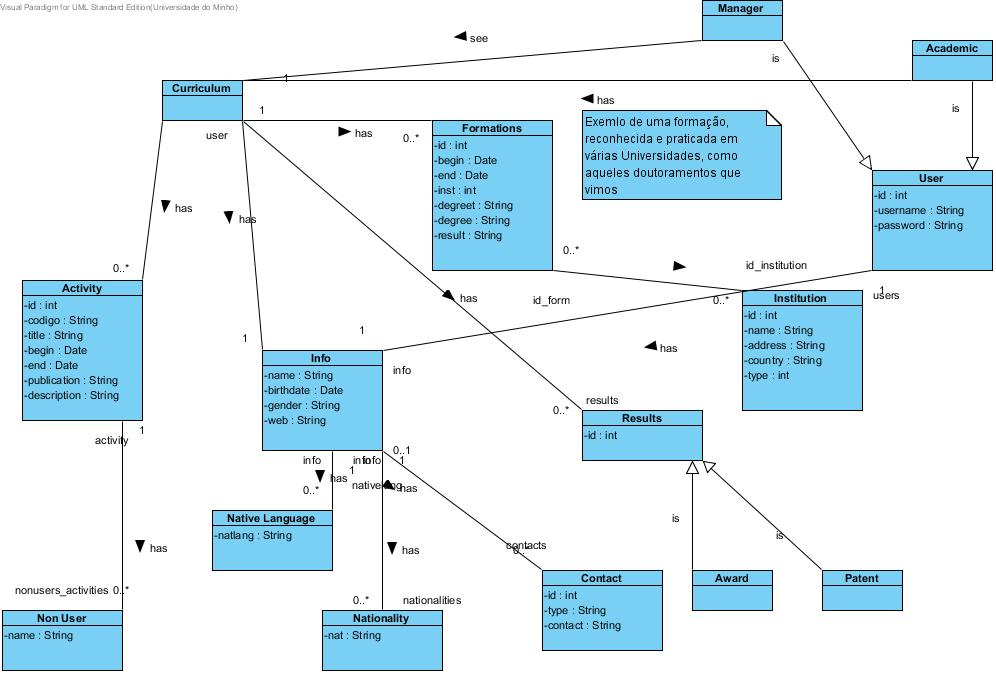
\includegraphics[scale=.4]{Diagrama_Classes.jpg}
\caption{Diagrama de Classes}
\label{fig:diagramadeclasses}
\end{figure}
O Diagrama de Classes, presente na figura \ref{fig:diagramadeclasses} inicialmente desenvolvido estava consideravelmente mais pobre e foi enriquecido também à medida que fomos avançando no projecto. Foi também um enorme ponto de partida para a criação da Base de Dados. A única parte ainda bastante subdesenvolvida é a dos resultados pelo facto de ainda não termos avançado muito nessa questão e ter ficado somente aquilo que retirámos das primeiras leituras, quer do enunciado, quer de exemplos facultados ou encontrados.
\subsection{Use Cases}
\begin{figure}[!ht]
\centering
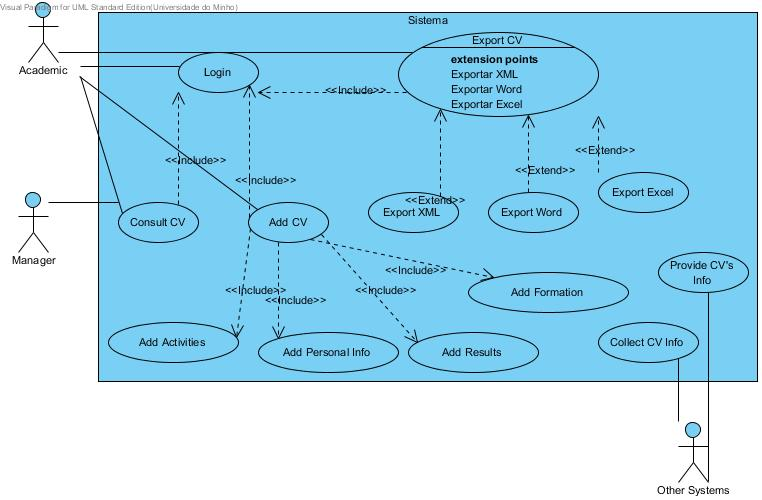
\includegraphics[scale=.6]{Use_Cases.jpg}
\caption{Use Cases}
\label{fig:usecases}
\end{figure}
Os \emph{Uses Cases} na figura \ref{fig:usecases} referem-se essencialmente a tarefas possíveis de serem feitas, quer pelo Gestor, quer pelo Académico (na maioria dos casos o académico será o docente).\\
Cada \emph{Use Case} possui uma descrição textual que nos permitiu já ponderar um pouco sobre como irá o sistema responder ao utilizador e interagir com outros sistemas. Podemos ver dois exemplos da descrição textual dos uses cases na figura \ref{fig:uc_consultcv} e \ref{fig:uc_providecvinfo}
\begin{figure}[!ht]
\centering
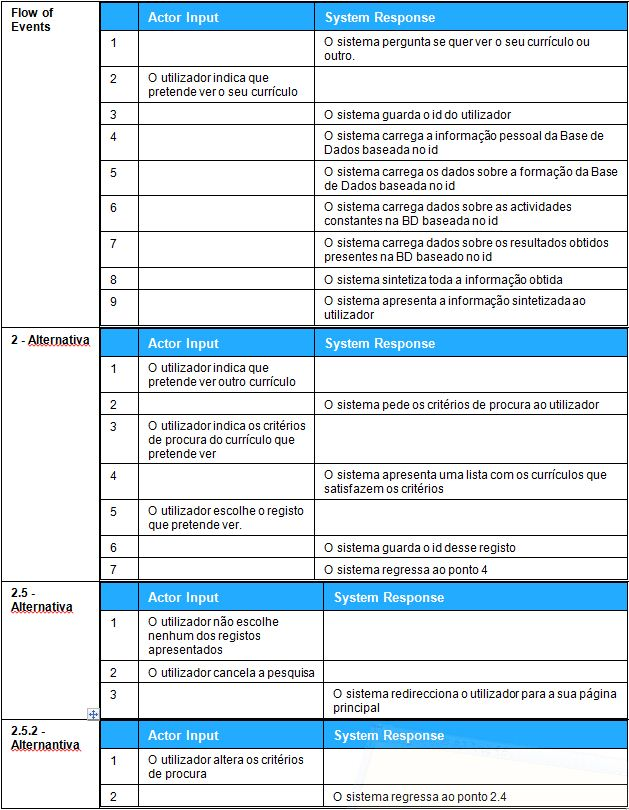
\includegraphics[scale=1]{uc_consult_cv.jpg}
\caption{Use Case - Consult CV}
\label{fig:uc_consultcv}
\end{figure}
\begin{figure}[!ht]
\centering
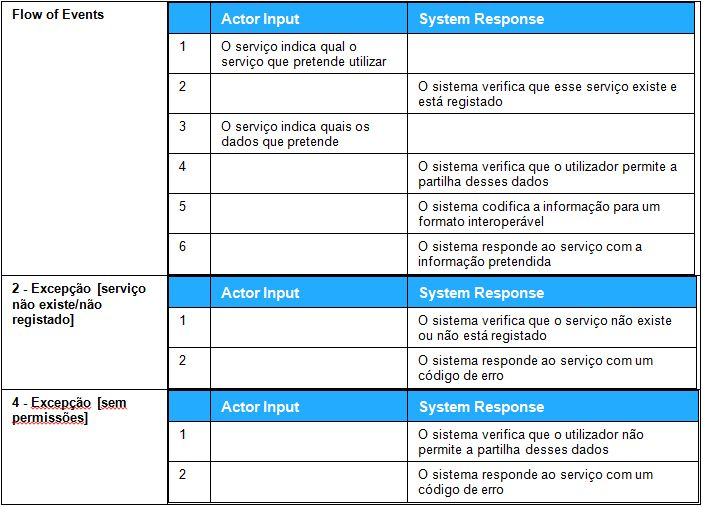
\includegraphics[scale=.9]{uc_provide_cv_info.jpg}
\caption{Use Case - Provide CV\rq{}s info}
\label{fig:uc_providecvinfo}
\end{figure}

\subsection{Base de Dados}
\begin{figure}[!ht]
\centering
\includegraphics[scale=1]{bd.eps}
\caption{1ª versão da Base de Dados}
\label{fig:basededados}
\end{figure}
A estrutura da base de dados (figura \ref{fig:basededados}) foi pensada de forma a permitir armazenar, como é óbvio, os dados que foram analisados por exemplo no diagrama de classes. Os seus relacionamentos foram facilmente idealizados.\\
Contudo no decorrer do projecto foi necessário proceder a algumas alterações na estrutura de Base de Dados de modo a corrigir alguns problemas detectados na fase da implementação dos vários importadores, como podemos ver na figura \ref{fig:basededados2}
\begin{figure}[!ht]
\centering
\includegraphics[scale=1]{bd2.eps}
\caption{2ª versão da Base de Dados}
\label{fig:basededados2}
\end{figure}
\section{Linguagem formal para Identificação e Formação}
\subsection{Gramática}
A Gramática para a linguagem de identificação e formação foi facilmente criada, recorrendo ao que já tínhamos analisado para o diagrama de classes. No entanto, permitiu-nos também enriquecer mais o diagrama de classes, pois ao irmos escrevendo a gramática lembramo-nos de coisas que nos poderiam fazer falta.\\
Apesar de tudo não refinámos ainda muito certos campos como o email e o web porque são coisas definidas por normas externas, que queríamos tentar seguir e adaptar à gramática desenvolvida no AntLR.\\
Também aqui decidimos fazer, que permita futuras actualizações em implicar uma completa reestruturação da gramática. Uma delas foi aquilo a que nos chamamos \emph{Special ID} (SPID), por exemplo para valores como o País. Isto porque o País é um cujo os valores podem ser normalizados de modo a que não existam dois países iguais com nomes diferentes, e poderá permitir mais para a frente se acharmos conveniente criar mais uma relação na Base de Dados, de modo a reduzir o espaço ocupado, por exemplo pelas nacionalidades.
\begin{verbatim}
SPID
	:	('A'..'Z')('a'..'z')* (' '('A'..'Z')('a'..'z')*)*
	;
\end{verbatim}
\subsection{Processador}
Quando discutimos o nosso processador, foi ponto assente, que queríamos evitar a repetição de código, assim sendo tentamos passar grande parte da responsabilidade para o ficheiro \emph{info\_import.php}, que seria um \emph{template}. Assim grande parte das coisas geradas pelo Parser seriam simplesmente valores etiquetados que ele saberia onde colocar.\\
Infelizmente não tivemos muito tempo para implementar a detecção de erros semânticos e assim, apesar de ele já detectar erros, como a data de início ser superior às de fim, apenas mostra essa mensagem mas continua o processamento.\\

O código de execução do \emph{parser} e leitura dos resultados também não é muito complexa. No entanto permite que estejam vários utilizadores simultâneos a executar a aplicação web, sem existir nenhum tipo de conflitos já que o \emph{stdout} é redireccionado para a leitura do php através de um \emph{handler}.
\begin{verbatim}
$f = (popen('java -jar AntLRParser.jar "'.$_FILES['ficheiro']['tmp_name'].'"', "r"));

$valor = "";
while (!feof($f)) {$valor .= fread($f, 60);}
\end{verbatim}
Depois as inserções são feitas na Base de Dados MySQL recorrendo à classe PDO do php.
\subsection{Exemplo de Input}
Aqui está um exemplo de \emph{input} válido para a gramática desenvolvida.
\begin{verbatim}
@info {
	Name: "Nelson José Costa Luís"
	Nationalities: [Portuguese, Canadian]
	PersonalContacts: [
					Email: nelson@uminho.pt,
					Phone: "259225225"
				  ]
	Birthdate: 03/05/1980
	Gender: M
	NativeLang: [Portuguese, English]
	Web: http://di.uminho.pt
}
@form {
	Begin: 15/09/1995
	End: 15/07/1998
	Institution:
		Name: "Universidade do Minho"
		Address: "Gualtar"
		Country: Portugal
		Type: Public University
	Degree: BSc "Engharia Informática"
	Result: 16
}
@form {
	Begin: 15/09/1998
	End: 15/07/2000
	Institution: 
		Name: "Universidade do Minho"
		Address: "Gualtar"
		Country: Portugal
		Type: Public University
	Degree: MSc "Engharia Informática"
	Result: 17
}
\end{verbatim}
\section{Linguagem de anotação para descrição das Actividades}
O \emph{Schema} (na figura \ref{fig:cv_activities}) desenvolvido para a descrição de actividades, teve também por modelo o que já tínhamos definido para a Base de Dados, para tentar equilibrar os dados que poderiam ser guardados e os que seriam enviados.\\
Um facto bastante relevante é permitir que uma actividade esteja relacionada com mais que um utilizador, podendo descrevê-lo como utilizador do sistema, ou não utilizador. No entanto o utilizador que está a submeter a informação sobre actividades não necessita de indicar directamente se o utilizador é ou não utilizador da plataforma. A própria plataforma, recorrendo a um script perl irá determinar com base na similaridade do nome apresentado, com os nomes totais dos utilizadores na plataforma, o utilizador a que se refere. No caso de conseguir um grau de probabilidade superior a 80\% no nome obtido, será considerado esse utilizador. Caso contrário será acrescentado como não utilizador da plataforma. Mas o utilizador que submeter terá sempre a possibilidade de alterar as suas referências a actividades. Também os outros utilizadores considerados parceiros nessa actividade podem optar por remover-se dessa mesma actividade.
\begin{figure}[!ht]
\centering
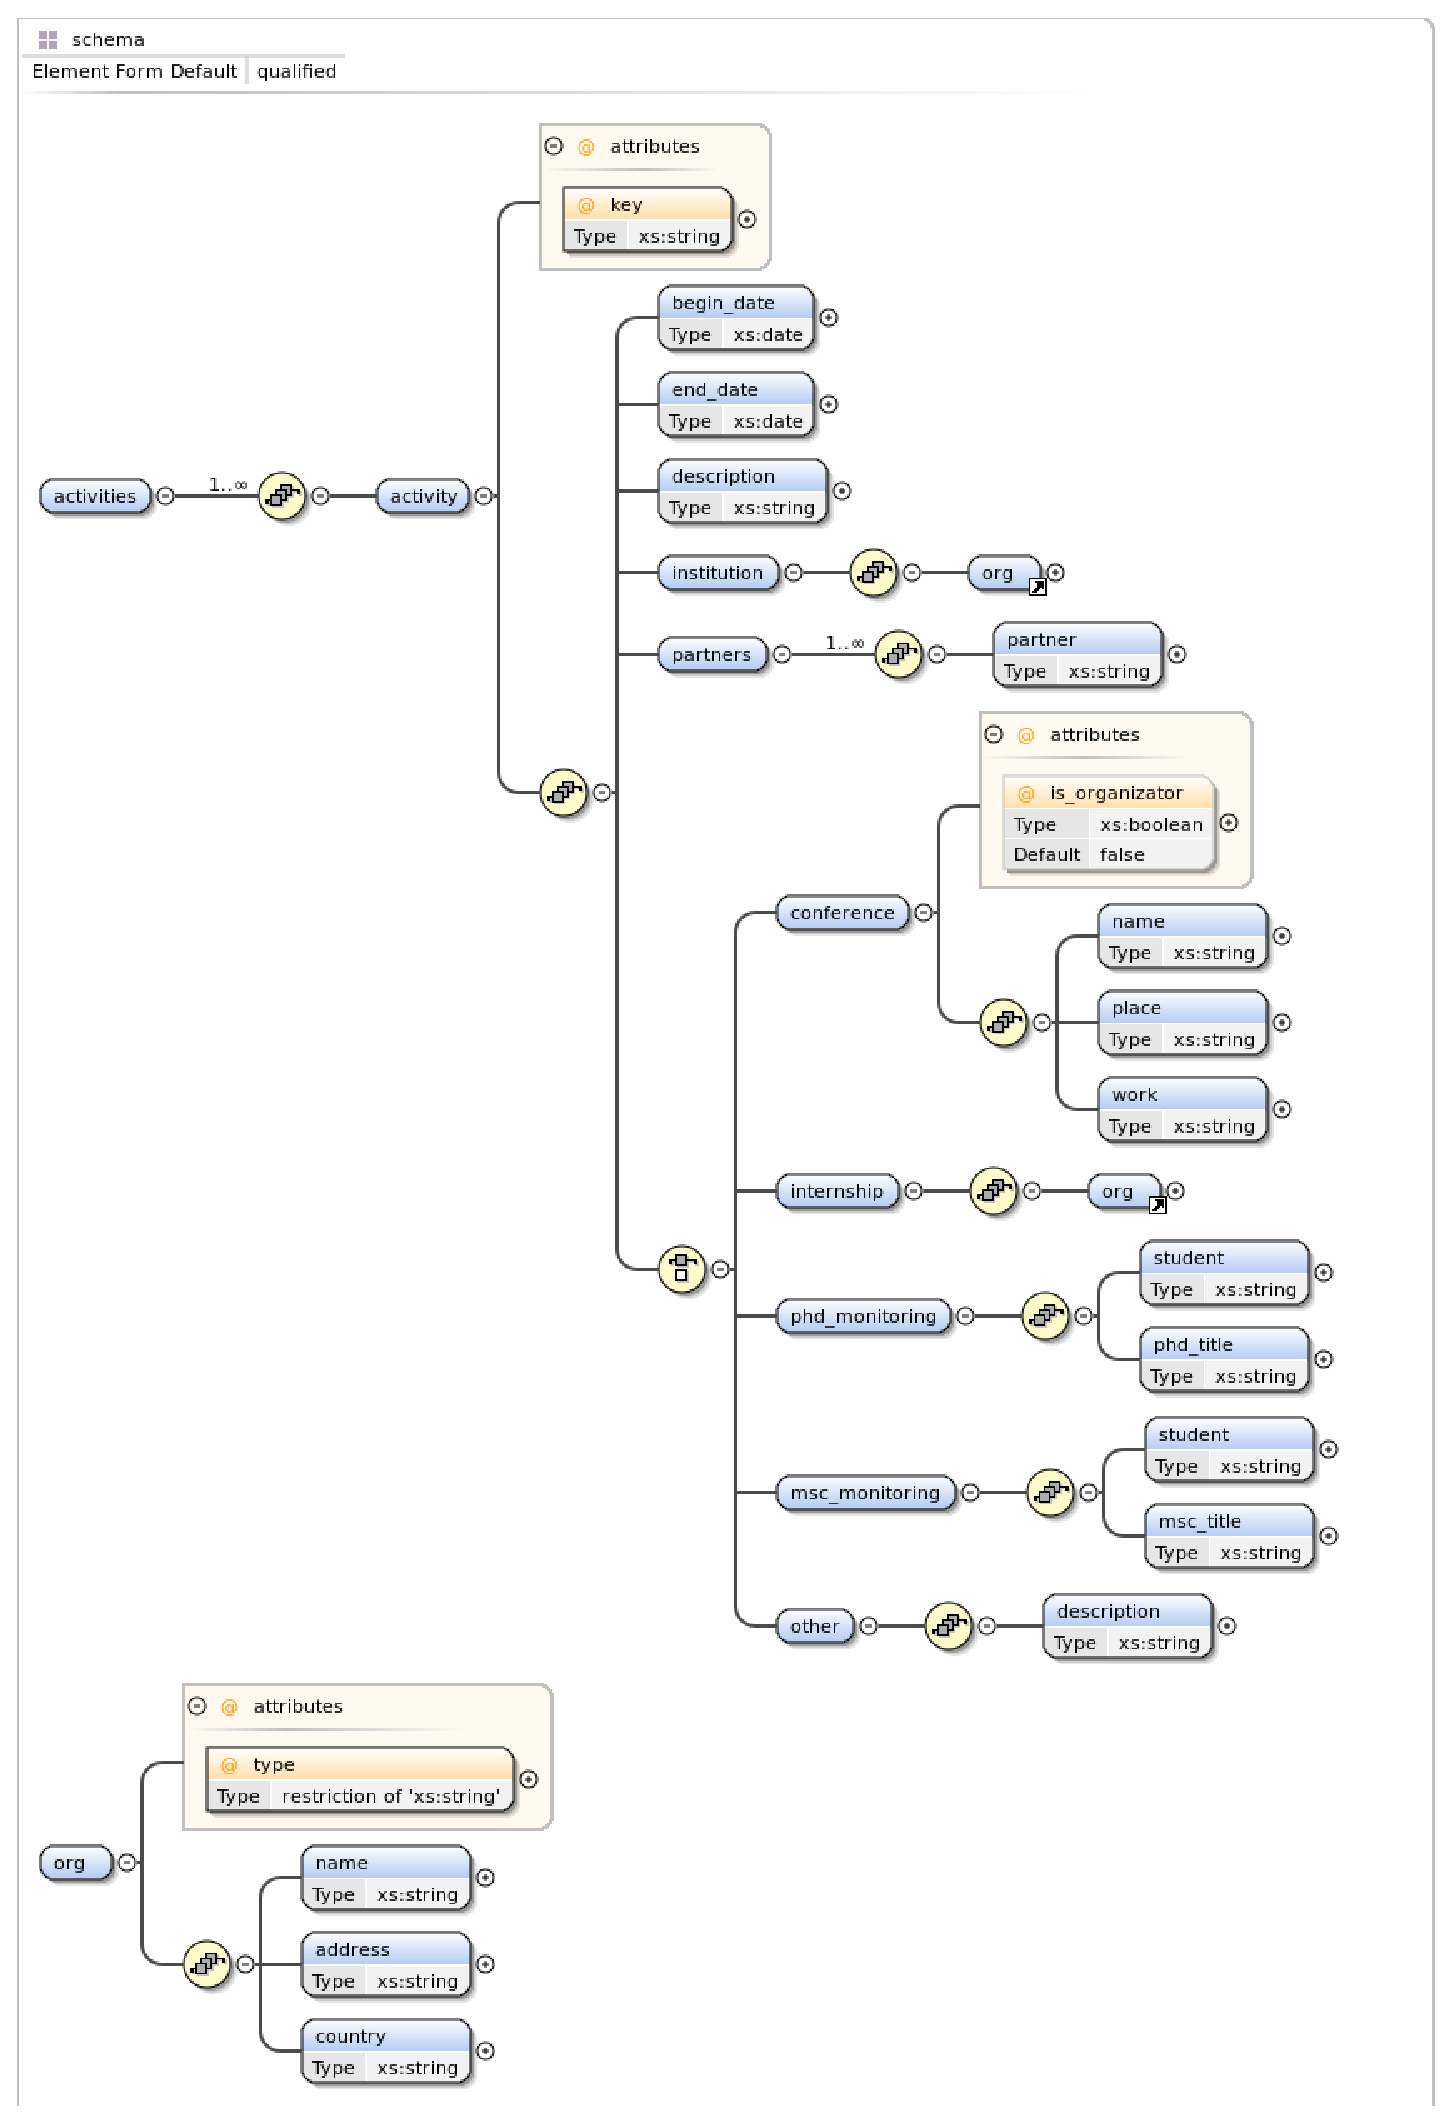
\includegraphics[scale=0.70]{cv_activities_schema.eps}
\caption{Schema da linguagem}
\label{fig:cv_activities}
\end{figure}

\subsection{Processador}
O processador para esta linguagem descrita pelo \emph{Schema} anterior foi desenvolvido em \emph{PHP} tendo em vista uma maior facilidade de manutenção e de criação. Poderíamos ter optado por algo como um \emph{XSL} mas isso obrigaria sempre a que a mesma gerasse ou código SQL, que seria depois utilizado por um script \emph{PHP}, ou então à geração do próprio código \emph{PHP}. Neste último caso o processamento seria mais extensivo porque primeiro teria que ser processado o \emph{XSL} e depois executado o \emph{PHP} por ele gerado. Por estes motivos, resolvemos utilizar as ferramentas disponíveis na linguagem de programação \emph{PHP}, como o \emph{DOMDocument} e o \emph{DOMXpath}. Inclusivamente para ser mais fácil o processamento extendemos ligeiramente a classe \emph{DOMXpath} como podemos ver no excerto de código a seguir:
\begin{verbatim}
   class myXPath extends DOMXPath{
        const RES = 'RETURNRES';
        public function queryValue($query, $node = null, $default = null){
            $res = $this->query($query, $node);
            if ($default === self::RES) return $res;
            if ($res === false || $res->length < 1){
                $aux = $default;
            }else if ($res->length > 1){
                $aux = array();
                foreach($res as $valor)
                    $aux[] = $valor->textContent;
            }else{
                $aux = $res->item(0)->textContent;
            }
            return $aux;
        }
        public function recQueryToArray($query, $node){
            $arr = array();
            $res = $this->query($query, $node);
            if ($res === false || $res->length <= 0) return false;
            foreach($res as $chave => $valor) {
                $aux = $this->recQueryToArray($query, $valor);
                if ($aux === false)
                    $arr[$valor->localName]['__text'] = $valor->textContent;
                else 
                    $arr[$valor->localName] = $aux;
                if ($valor->hasAttributes()){
                    $arr[$valor->localName]['__atributes'] = array();
                    $length = $valor->attributes->length;
                    for ($i = 0; $i < $length; ++$i) {
                        $atr = $valor->attributes->item($i);
                        $arr[$valor->localName]['__atributes'][$atr->name] = $atr->value;  
                    }
                }
            }
            return $arr;
        }
    }
\end{verbatim}
Questões como os partners, foram alteradas, de modo a que o utilizador não se preocupe se é ou não utilizador da plataforma, já que a mesma recorre a uma ferramenta criada maioritariamente nas aulas de \emph{SPLN}, com o intuito de desambiguar nomes
\subsection{Exemplo de Input}
\begin{verbatim}
<?xml version="1.0" encoding="UTF-8"?>
<activities>
  <activities key="ex1">
    <begin_date>01/01/2012</begin_date>
    <end_date>31/12/2012</end_date>
    <description>Exemplo de uma actividade</description>
    <institution>
      <org type="Public University">
        <name>Universidade do Minho</name>
        <address>Gualtar</address>
        <country>Portugal</country>
      </org>
    </institution>
    <partners>
      <partner>J. J. Almeida</partner>
      <partner>Bruno Fernandes</partner>
    </partners>
    <conference is_organizator="false">
      <name>JOIN - Jornadas de Informática da Universidade do Minho</name>
      <place>Universidade do Minho - Gualtar</place>
    </conference>
  </activities>
  <activities key="ex2">
    <begin_date>01/05/2011</begin_date>
    <end_date>31/06/2011</end_date>
    <description>Actividade de 2 meses</description>
    <institution>
      <org type="Private University">
        <name>Universidade Lusíada</name>
        <address>Famalicão</address>
        <country>Portugal</country>
      </org>
    </institution>
    <partners/>
    <other>
      <description>Exemplo de uma actividade mais específica que deve ser descrita pelo utilizador</description>
    </other>
  </activities>
</activities>
\end{verbatim}

\section{Formato standard para descrição de publicações}
Para a leitura dos ficheiros \textsc{Bib}\negthinspace\TeX optamos por uma script em perl. Na verdade, esta script está implementada como um módulo, usando, portanto, as capacidades OO do perl. A nível de implementação e para facilitar o desenvolvimento inicial, módulos alternativos como o Moose ou o Moo, os quais tentam implementar as \textit{features} OO do perl 6 foram considerados. No entanto, dado o overhead considerável que estes módulos têm, estes foram descartados e optamos por uma via mais convencional. De notar que foi feito algum esforço para que este módulo fosse o mais genérico, de forma a facilitar eventuais alterações futuras.  Esta script aceita como parâmetros de entrada o ficheiro que é suposto processar, bem como as credenciais da Base de Dados à qual se deve ligar. De seguida, o método \textit{parse} recebe o tipo de publicação a ser processado (article, techreport ou inproceedings). O resto acontece internamente e os dados são colocados numa hash organizada por autor. Por fim, basta chamar o método \textit{insertDB} e os dados são inseridos na base de dados. Obviamente que esta é a parte menos genérica do módulo, pois o schema da base de dados não pode ser definido em run-time, a não ser que se criasse uma Base de Dados apenas para este efeito. 

\subsection{Processador}
Dada a extensão do módulo, segue, apenas, o processamento de um article bem como a sua inserção na base de dados.

\begin{verbatim}
foreach (@bib) {                    
    
    $found = 1 if $_ =~ /\@article.*/;
    
    if($found) {

      if ($_ =~ m/^\}$/) {
        $found = 0;
        $self->{entries} += 1;
        foreach (@authors) {
          if (!defined $self->{parsedInfo}->{$_}) {
            $self->{parsedInfo}->{$_} = [];
            push $self->{parsedInfo}->{$_}, ["article",$title, $journal,$year];
          }
          else {
            push $self->{parsedInfo}->{$_}, ["article",$title, $journal,$year]; 
          }
        }

        for my $i (0 .. $#authors) {
          delete $authors[$i];
        }         
      }       

      if ($_ =~ /author\s*=\s*(?:\{|\")(.*)(?:\}|\")/) {                                        
        my @tmp = split /and/, $1;

        for my $name (@tmp) {
          push @authors, trim($name);       
        }               
      }

      if ($_ =~ /title\s*=\s*(?:\{|\")(.*)(?:\}|\")/) {       
        $title = $1;
      }

      if ($_ =~ /journal\s*=\s*(?:\{|\")(.*)(?:\}|\")/) {       
        $journal = $1;
      }

      #year = {num}
      if ($_ =~ /year\s*=\s*(?:\{|\")(.*)(?:\}|\")/) {        
        $year = $1;
      }

      #year = num
      if ($_ =~ /year\s*=\s*(\d+)/) {       
        $year = $1;
      }                                         
      
    }   
  }
\end{verbatim}
Inserção na BD:\\
\begin{verbatim}
  for my $aut (keys $res) {
    if ($aut eq $user) {
      $found = 1;
      last;
    }
  }
  return NO_USER if not $found;


  my $sth = $dbh->prepare("select * from info where name = ?");
  $sth->bind_param(1,$user);
  $sth->execute;

  while (my @tmp = $sth->fetchrow_array()) {
    $usr_id = $tmp[0]; #fetch user id
  }
  $res = $res->{$user};
  my $id;

  foreach (@$res) {   
    my @arr = @$_;      
    if ($arr[0] eq 'article') {
      $sth = $dbh->prepare("insert into publications  (`type`, `title`, 
            `journal`, `year`) values (?,?,?,?)");
      $sth->bind_param(1,$arr[0]);
      $sth->bind_param(2,$arr[1]);
      $sth->bind_param(3,$arr[2]);
      $sth->bind_param(4,$arr[3]);            
      $sth->execute;
      $id = $dbh->{ q{mysql_insertid}};

      $sth = $dbh->prepare("insert into users_publications values ($usr_id,$id)");
      $sth->execute;
    }
\end{verbatim}
  

\subsection{Exemplo de Utilização}

\begin{verbatim}
  my $f = BibTeX::toDB->new('bibtex.bib','DBI:mysql:database','user','pass');

  $f->parse("article");
  $f->parse("techreport");
  $f->parse("inproceedings");
  $f->insertDB("J.J. Almeida");
\end{verbatim}

\section{Interface única para carregamento dos vários dados relativos ao CV}
A nossa interface para o carregamento dos dados, permite de forma bastante interactiva introduzir os dados referentes à informação básica, formação e actividades desenvolvidas. Atendendo a que o ficheiro de publicações é um simples ficheiro BibTeX, e já existem uma quantidade razoável de ferramentas que permite criar esses mesmos ficheiros, apenas temos o local de colocação de um ficheiro. No entanto a interface possui algumas simplificações, mas que podem ser limitativas para alguns CVs. Por isso mesmo é permitida a introdução de um ficheiro único, com todas as informações. Esse ficheiro, mais não é que um zip, contendo um manifesto (\emph{pr.xml}) que indica quais os ficheiros dentro do pacote que se referem à informação e formação, às actividades e às publicações. Para melhor comodidade podem haver mais que um ficheiro para cada uma das categorias (sendo que todos serão processados). Podemos ver um exemplo de um manifesto de um pacote:
\begin{verbatim}
<?xml version="1.0" encoding="UTF-8"?>
<cv>
  <info>
    <file>info.txt</file>
    <file>formation.txt</file>
  </info>
  <activities>
    <file>act.xml</file>
    <file>act2.xml</file>
  </activities>
  <publications>
    <file>pub.bib</file>
  </publications>
</cv>
\end{verbatim}
No caso da primeira e terceiras partes o conteúdo dos vários será concatenado e depois processado pelo processador respectivo. No caso da segunda parte, das actividades, cada xml será tratado de forma independente (lido e verificado um a um, sem nenhum tipo de concatenação).\\
\subsection{Imagens da interface}
Podemos observar três imagens referentes aos campos disponíveis para cada secção, relativamente à informação recolhida. A figura \ref{fig:bypacote} dá a possibilidade de ser submetido directamente um ficheiro zip com todas as informações directamente lá contidas, ao mesmo tempo que garante uma maior flexibilidade.\\
Podemos ver como no entanto é possível a interface adequar-se, por exemplo a cada tipo de actividade, garantindo uma maior capacidade ao utilizador de saber que campos serão realmente necessários.
\begin{figure}[!ht]
\centering
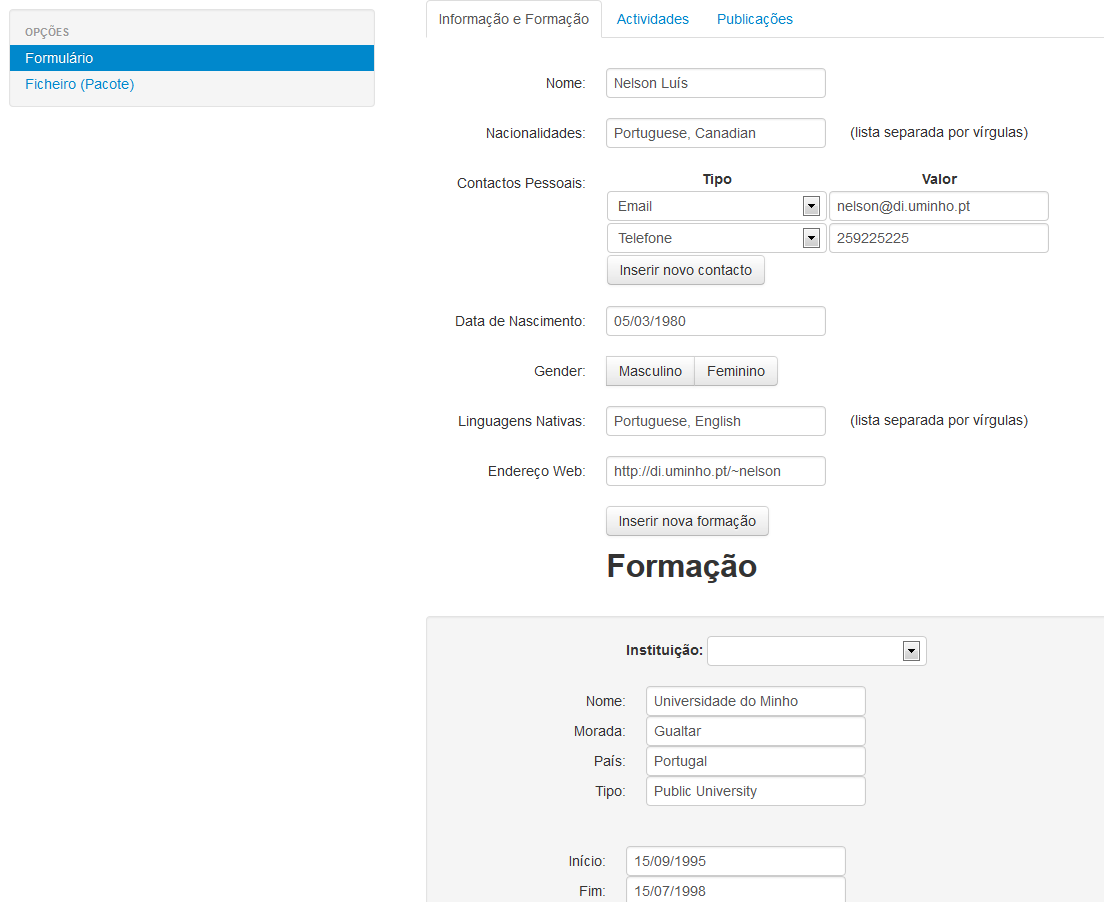
\includegraphics[scale=0.6]{iInfo.png}
\caption{Formulário para introdução da informação básica e formação}
\label{fig:iinfo}
\end{figure}
\begin{figure}[!ht]
\centering
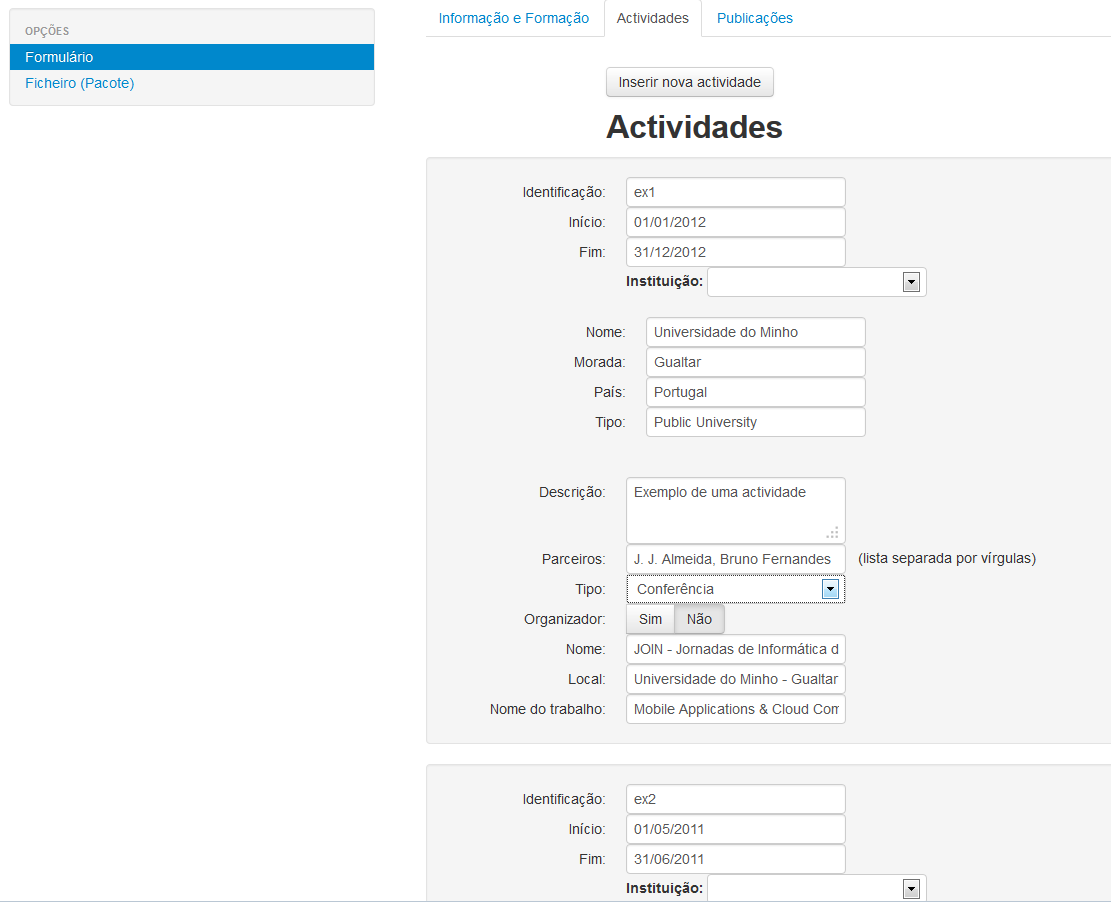
\includegraphics[scale=0.6]{iActivities.png}
\caption{Formulário para introdução das actividades desenvolvidas}
\label{fig:iActivities}
\end{figure}
\begin{figure}[!ht]
\centering
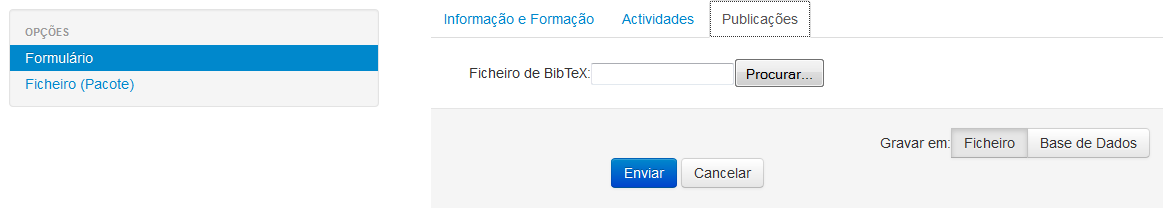
\includegraphics[scale=0.6]{iPublications.png}
\caption{Formulário para introdução das publicações}
\label{fig:iPublications}
\end{figure}
\begin{figure}[!ht]
\centering
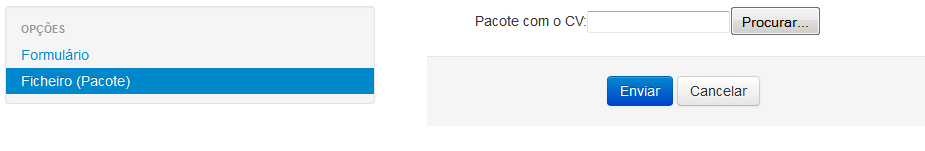
\includegraphics[scale=0.6]{bypacote.png}
\caption{Formulário para introdução do pacote em formato zip}
\label{fig:bypacote}
\end{figure}

\section{Conclusão}
O objectivo desta segunda avaliação do Projecto Integrado, é garantir que o mesmo segue já a um bom ritmo, servindo também já como um suporte para o desenvolvimento futuro, na medida em que será uma base sobre a qual podemos continuar a construir já mais cientes dos caminhos correctos que escolhemos e daqueles que não estavam assim tão correctos, ao ser mostrado à equipa docente os resultados obtidos até à data. Ao mesmo tempo confrontámos também as alterações que fizemos fruto da primeira avaliação, e das opiniões dos docentes.
\end{document}